\section{Agent-Oriented Planning in Multi-Agent Systems}
\label{sec:method}
In this section, we introduce the details of the proposed \name framework, with the overall architecture illustrated in Figure~\ref{framework}.


\begin{figure}[!t]
\centering
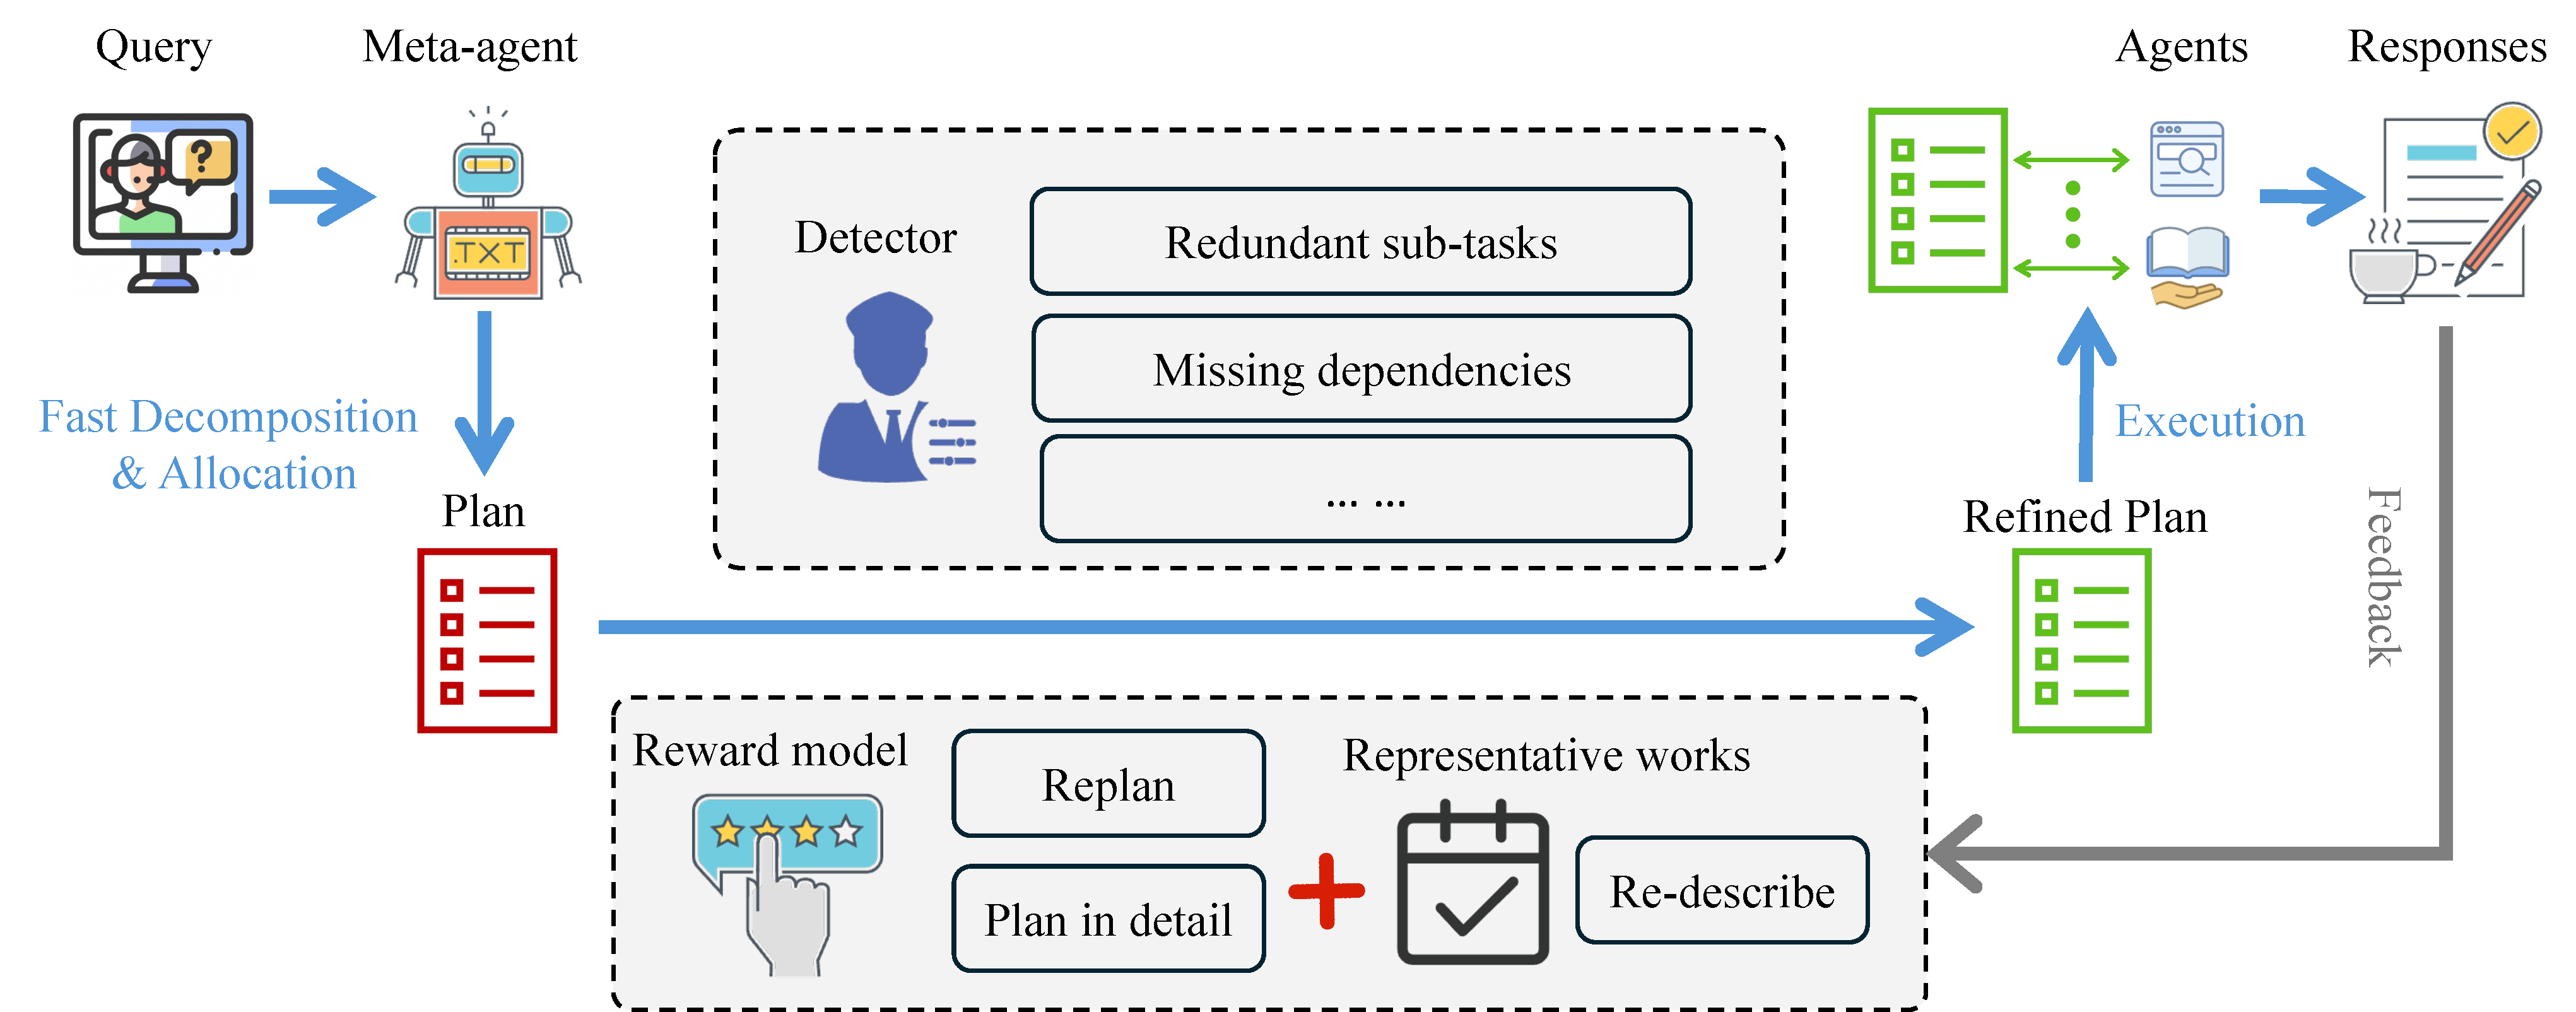
\includegraphics[width=0.95\linewidth]{figure/overall.pdf}
\caption{Overall architecture of \name. The framework begins with the {\it meta-agent} performing a fast decomposition and allocation of the received user query, resulting in an initial plan. A {\it detector} is employed to improve the completeness and eliminate redundancy of the plan, while a {\it reward model} provides scores to guide the meta-agent in refining the plan further, which involves operations such as replan, plan-in-detail, etc. The refined plan is sent back to the multi-agent system for generating responses to the user query.}
\label{framework}
\end{figure}


\subsection{Fast Decomposition and Allocation}
\label{subsec:fast_decompose}
First of all, following existing studies~\citep{shen2024hugginggpt, chen2023autoagents}, we provide detailed instructions to the meta-agent to guide it in performing agent-oriented planning. What sets our approach apart is that the provided instructions incorporate the following requirements:
(i) Integration of the user query $Q$ and all the agent descriptions $\mathcal{D}$: We include both the user query and the agents' descriptions in the instructions, promoting the meta-agent to fully consider the capabilities of each agent and tailor the sub-tasks to align with these capabilities. 
(ii) Suggestions for assigned agents: We require the meta-agent to provide suggestions for the agents assigned to each decomposed sub-task. Although we tend to separate task decomposition and assignment into two independent tasks performed sequentially, the experimental observations indicate that combining these two tasks enhances the effectiveness of agent-oriented planning. 
(iii) Structured decomposition of tasks: The decomposed tasks are required to be structured in a sequential manner, specifying any dependencies that may exist between sub-tasks, which ensures that the execution of tasks follows a correct logical order.
The adopted prompt can be found in Appendix~\ref{app_meta-agent}.

The aforementioned process of agent-oriented planning, which is called {\it fast decomposition and allocation} in this study, heavily relies on the capabilities of the meta-agent and meticulously designed system prompts. While such an end-to-end approach can achieve high efficiency, its success rate, namely fulfilling the three design principles mentioned above and providing reliable answers to the original user query, and its stability, namely the meta-agent can follow instructions and produce formatted responses, might not be satisfactory.

Inspired by recent studies on inference time computing~\citep {openai20244o}, we propose to design mechanisms to guide the meta-agent toward more comprehensive reasoning processes. The results of fast decomposition and allocation should be viewed as intermediate outputs rather than final results, which need to be further evaluated to offer detailed revision suggestions for the meta-agent. 
More details on this proposed approach are provided in the next subsection.


\subsection{Is A Sub-Task Completely Resolved?}
\label{subsec:reward_model}
To determine whether a sub-task can be resolved by a single agent, i.e., satisfying the principle of solvability, a straightforward solution is to send the sub-task to every agent in the system. Each agent generates a response to the sub-task, allowing us to select the best answer and assess whether it completely resolves the sub-task.
However, this approach is often impractical due to the unaffordable overhead. For a user query decomposed into $m$ sub-tasks, a multi-agent system with $n$ agents would need to execute a total of $m\times n$ agent calls for just a single trial, making it an inefficient strategy in scenarios with a large number of agents and sub-tasks.

To tackle this, we introduce a reward model that provides efficient evaluations of the solvability of sub-tasks, which aims to predict the quality of the agents' responses to sub-tasks without necessitating actual agent calls.

Specifically, we first prepare a dataset for training the reward model. 
For a given user query $Q$, we follow the fast decomposition and allocation process introduced in Section~\ref{subsec:fast_decompose}, requiring the meta-agent to decompose $Q$ into several sub-tasks and select $l$ agents for each sub-task based on the agents' descriptions, 
which can be formally given as follows:
\begin{equation}
 \mathcal{P}(Q, \mathcal{D}, \mathcal{A})=\{(q_i, \mathcal{A}_{i,1},...,\mathcal{A}_{i,l})\ |\ i\in[m]\}.
\end{equation} 
After that, we execute the plan, i.e., sending the sub-tasks to the assigned agents, and obtain all the responses from agents as:
\begin{equation}
\{r_{i,j}=\mathcal{A}_{i,j}(q_i)\ |\ i\in[m], j\in[l]\},
\end{equation}
where the choice of $l$ can be a trade-off. A large $l$ leads to comprehensive responses from lots of agents for constructing the training dataset, while it might need more computation resources and affect the overall quality of the dataset. In this study, we set $l$ to be half the number of agents in the multi-agent systems.

We utilize a scorer $\mathcal{S}$ that evaluates agents' responses to sub-tasks, i.e., $\mathcal{S}(q_i,r_{i,j})=s_{i,j}$, which serves as annotations in the training dataset.
The scorer $\mathcal{S}$ provides evaluations from three key aspects, including correctness, relevance, and completeness, and can be implemented by using LLMs or employing human annotators.
We apply this scoring process across a diverse array of user queries $\mathcal{Q}=\{Q_k\}_{k=1}^K$ and collect the results to form the training dataset, denoted as $\mathcal{T} = \{(q_{k,i}, d_{k,i,j},s_{k,i,j})\ |\ k\in[K],i\in[m_k],j\in[l]\}$.
More details on the construction of the dataset, such as the adopted prompts, are summarized in Appendix~\ref{training}. 

The reward model $\mathcal{M}$, parameterized as $\theta$, consists of embedding layers followed by fully connected layers. We obtain embeddings for both the sub-task and the agent's description separately, then concatenate these embeddings together and feed them into the fully connected layers for further processing.
To provide evaluations without making actual agent calls, we design the training objective aimed at minimizing the discrepancies between the model's predictions and the annotations provided by the scorer, which can be formulated as follows:
\begin{equation}
    L(\mathcal{T}, \theta)=\frac{1}{K}\sum_{k=1}^K\frac{1}{m_k}\sum_{i=1}^{m_k}\frac{1}{l}\sum_{j=1}^l(s_{k,i,j}-\mathcal{M}_\theta(q_{k,i}, d_{k,i,j}))^2.
\end{equation}

With the well-trained reward model, the evaluation of the results produced by fast decomposition and allocation can be summarized as follows. For each suggestion provided by the meta-agent, stating the assignment of sub-task $q_i$ to agent $\mathcal{A}_i'$, the reward model predicts a score denoted as $\mathcal{M}_\theta(q_i, d_i')$. A sufficiently high predicted score, which implies that $q_i$ can be completely resolved by agent $\mathcal{A}_i'$, leads to the acceptance of this suggestion. Conversely, if the predicted score falls below a predefined threshold, which indicates that the assignment should be revisited by the meta-agent, the reward model provides a set of scores $\hat{s}_{i,j}=\mathcal{M}_\theta(q_i, d_j)$ for all the agents $\mathcal{A}_j, j=1,...,n$. From these scores, the meta-agent reports the optimal selection as $j_{max}=\mathrm{argmax}_j\,\hat{s}_{i,j}$.

Note that there may be scenarios where the highest score $\hat{s}_{i, j_{max}}$ is still extremely low, indicating that the sub-task $q_i$ does not satisfy the principle of solvability and that no single agent can resolve it independently. In these cases, the meta-agent $\mathcal{P}$ is required to perform a {\it replan} on $q_i$.
The prompt used for replan is detailed in Appendix \ref{app_replan}.





\subsection{Sub-Task Modifications}
\label{subsec:task_modifications}
In addition to the two scenarios mentioned in Section~\ref{subsec:reward_model}, where the assignment of sub-task $q_i$ to agent $\mathcal{A}_i'$ is either predicted to be acceptable by the reward model or to be entirely inappropriate and requires a replan process, there also exists another situation where agent $\mathcal{A}_i'$ might not provide a reliable response to sub-task $q_i$, even though the assignment seems reasonable according to the reward model.

We identify two intrinsic reasons for such a situation in agent-oriented planning.
First, the description of the sub-task may lack critical information necessary for solving the problem, such as the interpretation of contextual elements like pronouns or other ambiguous terms. In such cases, while the agent possesses the capability to resolve the sub-task, the missing information can hinder it from providing a satisfactory response.
Second, the sub-task $q_i$ might be too complex, therefore a single agent can only address parts of this sub-task based on its expertise and tools. 
In this subsection, we design mechanisms to distinguish between these two cases and propose corresponding solutions. 

To be more specific, for each agent, we propose to construct a set of representative works that record the sub-tasks it has completely resolved. We would initially bypass the construction and update for these representative works (refer to Section~\ref{subsec:feedback_loop} for more details) and focus on how to utilize them to make sub-tasks modifications here.
Given a sub-task $q_i$, we calculate its similarity with a representative work $q_t$ following $cos(\mathcal{E}(q_i), \mathcal{E}(q_t))$, where $\mathcal{E}$ is the embedding part in $\mathcal{M}$ and $cos(u,v) = \frac{u\cdot v}{\left\|u\right\|_2\left\|v\right\|_2}$ calculates the cosine similarity. We define the similarity as follows:
\begin{equation}
sim(q_i, \mathcal{Q}_j)=\max\{cos(\mathcal{E}(q_i), \mathcal{E}(q_t))|q_t\in \mathcal{Q}_j\},
\end{equation}
where it can be denoted as $sim_{i,j}$ for short. 

A large $\max\{sim_{i,j}\ |\ j\in[n]\}$ indicates that the representative works of the agent corresponding to $\max\{sim_{i,j}\ |\ j\in[n]\}$ contain a sub-task similar to $q_i$. Such a case should be attributed to the first reason mentioned above, and we tend to request the meta-agent to perform {\it re-describe} on $q_i$ according to the similar representative work.

On the other hand, when the calculated similarity does not meet the threshold, we regard $q_i$ as too complex for any single agent in the system to solve (corresponding to the second reason above). As a result, the meta-agent $\mathcal{P}$ is requested to perform {\it plan-in-detail} for further decomposing the sub-task into simple ones.
To avoid creating redundant sub-tasks, we provide $\mathcal{P}$ with all the sub-tasks and explicit instruction on avoiding overlapping sub-asks. The prompt used for sub-task modification can be found in Appendix~\ref{app_plan_in_detail} and Appendix~\ref{app_redescribe}.



\subsection{Detector for Completeness and Non-Redundancy}
\label{subsec:detector}
Following the idea in fast decomposition and allocation, we attempt to incorporate detailed instructions to the meta-agent to satisfy the principles of completeness and non-redundancy.
However, empirical observations reveal that these instructions may not always work well. In fact, more than 15\% of user queries still exhibit such issues during decomposition in our initial experiments.

To tackle these issues, we involve a detector, implemented by providing a role-play prompt to LLMs, to evaluate both the completeness and non-redundancy of the intermediate results provided by the meta-agent.
For the principle of completeness, the detector extracts all key elements and requirements from the original query and then matches these elements against each sub-task, determining whether the sub-tasks collectively address all essential aspects of the original task. 
To further ensure that each sub-task can be successfully executed, the detector is also required to determine whether there are any additional dependencies needed beyond those identified during decomposition (e.g., unforeseen dependencies). If such dependencies exist, the execution results of these dependent sub-tasks should also be provided as inputs.


Regarding non-redundancy, the detector is responsible for analyzing whether any two subtasks contain identical information or try to solve the same problem, and whether there are unnecessary subtasks that do not contribute to the user query's solution.

When the provided results do not satisfy the principles of completeness or non-redundancy, the detector identifies the missing key information or redundant content and offers recommendations for refining the plan, such as suggestions for supplementing missing details or removing overlapping sub-tasks. 
The prompt used for the detector is provided in Appendix~\ref{app_detector}.
From the experimental results shown in Table~\ref{ablation}, we observe that the detector effectively mitigates the issues of incompleteness and redundancy, leading to an effective and efficient agent-oriented planning process. 


\subsection{Feedback Loop}
\label{subsec:feedback_loop}

An automatic feedback loop is integrated into \name, promoting the ongoing enhancement of the problem-solving process.
As introduced in Section~\ref{subsec:reward_model}, the reward model can identify certain sub-tasks as being resolvable by specific agents.
These identified sub-tasks are then collected to form the {\it representative works} of the corresponding agents. The training data for the reward model, which includes the sub-tasks and the ground truth scores of responses provided by the agents, is utilized to initialize these representative works.

Note that the representative works are continuously updated. When a user query is completely resolved, the sub-tasks decomposed from that user query can be added to the representative works of the agents who are selected to provide responses to these sub-tasks.
To prevent redundancy in the representative works, we implement a similarity threshold. This threshold ensures that only new and sufficiently distinct sub-tasks are incorporated into an agent's representative works, maintaining the diversity and relevance of the tasks that each agent has previously resolved.



